\documentclass{llncs}

\usepackage[english]{babel}
\usepackage[tight]{subfigure}
% \usepackage{floatrow}
\usepackage{epsfig}
\usepackage{amsmath}
\usepackage{multirow}
\renewcommand*\arraystretch{1.25} % extra vertical space in cells

\begin{document}

\title{A Shell Model for Real-Time Simulation of Intra-ocular Implant Deployment}
\author{Olivier Comas, St\'ephane Cotin and Christian Duriez}
\institute{INRIA, Alcove team, Lille, France}

\maketitle

\begin{abstract}
With 30 million interventions a year worldwide, cataract surgery is one of the most frequently performed procedures. Yet, no tool currently allows teaching all steps of the procedure without putting patients at risk. A particularly challenging stage of this surgery deals with the injection and deployment of the intra-ocular lens implant. In this paper we propose to rely on shell theory to accurately describe the complex deformations of the implant. Our approach extends the co-rotational method used in finite element analysis of in-plane deformations to incorporate a bending energy. This results in a relatively simple and computationally efficient approach which was applied to the simulation of the lens deployment. This simulation also accounts for the complex contacts that take place during the injection phase. 
%Particular care was given to the validation of the proposed model, its computational efficiency and stability. 
\end{abstract}

\section{Introduction}
According to the latest assessment of the World Health Organization, age related cataract is responsible for $48\,\%$ of world blindness, which represents about 18 million people. Cataract is the clouding of the lens of the eye which impedes the passage of light. Its treatment is a surgical operation, where the opaque lens is removed and replaced by an artificial intra-ocular lens. As people live longer, more surgical interventions are needed. However, current methods of teaching are not compatible with increasing demands of training for this procedure, and also expose patients to complications inherent to the inexperience of the operator. A cataract surgery simulator can offer an efficient alternative teaching method for ophthalmologists, as illustrated in recent reports such as \cite{Feudner09}. The work presented in this paper focuses on the simulation of a crucial step of cataract surgery: the injection and deployment of an artificial lens. To reach this objective, we propose an efficient yet simple formulation for triangular shells, as well as a physically accurate model of the complex (self-)contacts that occur during the injection and deployment of the artificial lens. 

\subsection{Related work}

Although various shapes of intra-ocular lens implants exist they all share common properties: they are three-dimensional structures, usually made of acrylic
%\footnote{acrylic is the common name for polymethylmethacrylate} 
material, and are much thinner in one direction ($0.13$\,mm) than in the two other ones ($6$ and $13$\,mm). This last characteristic is what classifies these lenses as thin objects, i.e. three-dimensional objects that can be abstracted as two-dimensional structures. Numerous models are available in the literature to describe physics of thin objects, from fairly simple and naive approaches to more complex and thorough representations. Continuum mechanics provides many formulations able to accurately describe stresses occurring within thin objects. Most of them fall into one of the following two categories: plate theory or shell theory. Those theories have been a subject of interest in the mechanical community for decades. The difference between these two kinds of structures is very well explained by Liu \textit{et al.}~\cite{Liu03} and can be summarized by the fact that plate bending elements can only carry transversal loads while shells can undergo more complex deformations. 
For instance, if we consider the horizontal board of a bookshelf, that board can be approximated as a plate structure and the transversal loads are the weight of the books. A typical deformation of the board is illustrated in figure~\ref{fig-boards} left. Conversely, a shell structure can carry loads in all directions, and therefore can undergo bending, twisting and in-plane deformation (see Figure~\ref{fig-boards} right). 
Considering the folded shape of the implant within the injection device (see Figure \ref{fig-surgery}), a thin plate model would not correctly capture the deformation and therefore a shell formulation was retained to model the intra-ocular lens behaviour. 

\begin{figure}[ht]
\begin{center}
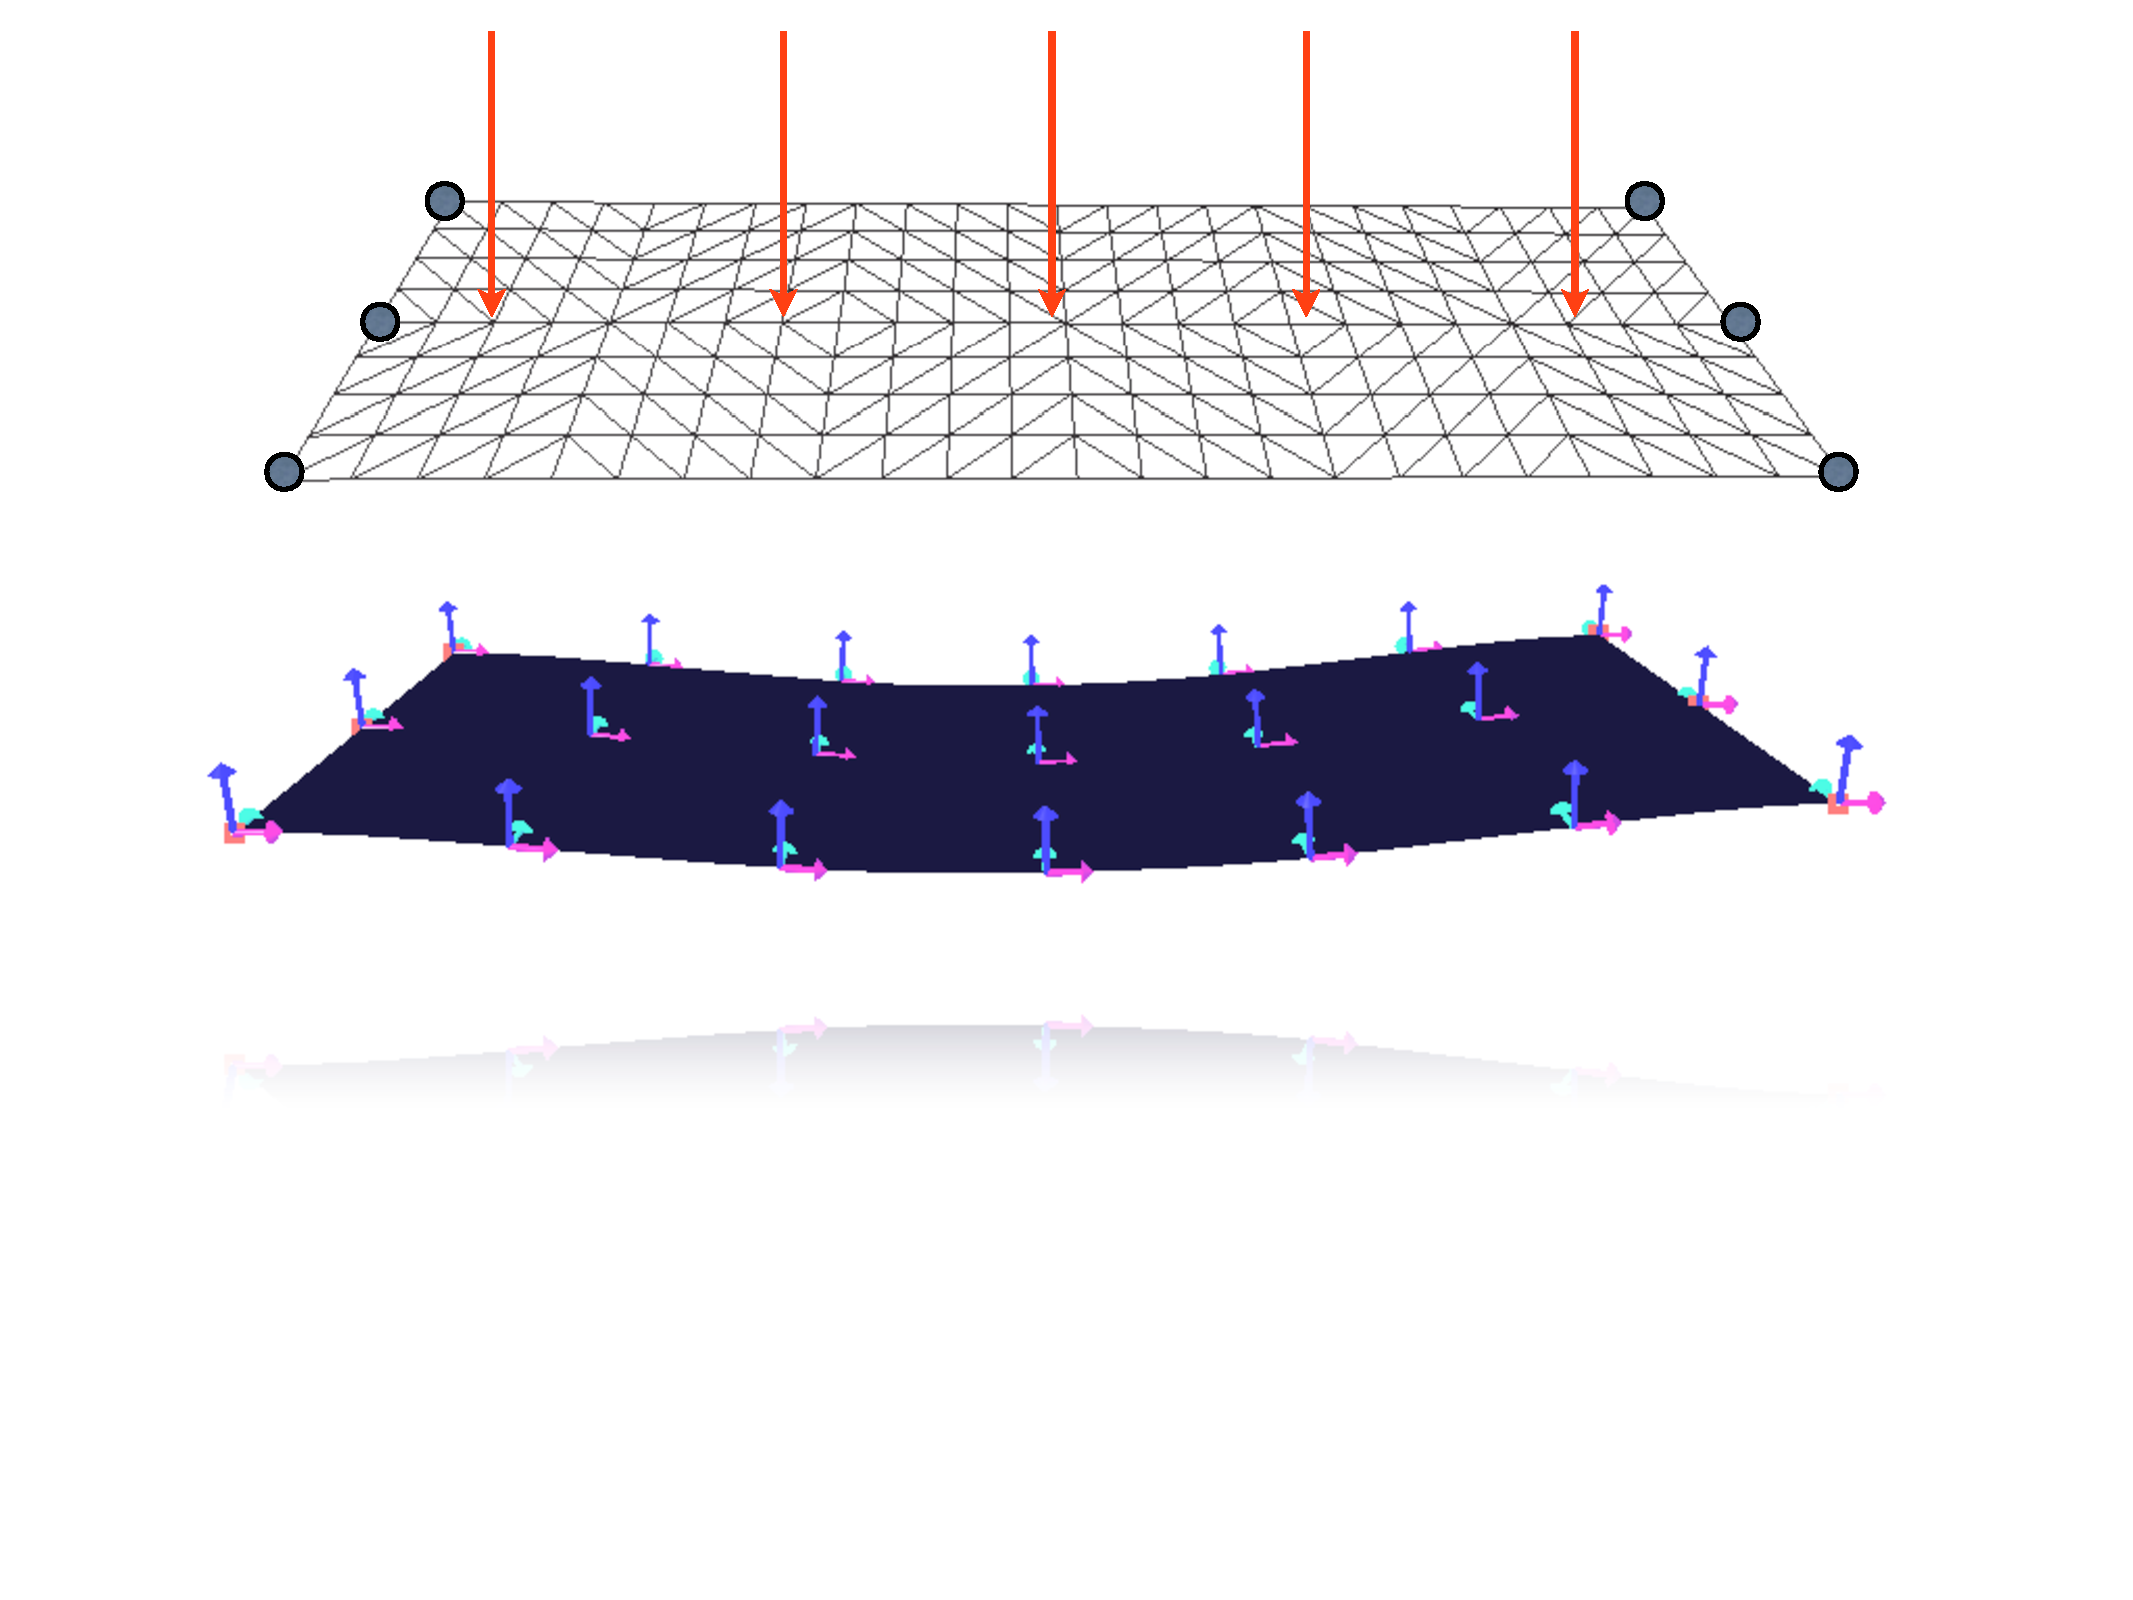
\includegraphics[width=6cm]{images/board_bending}
\hfill
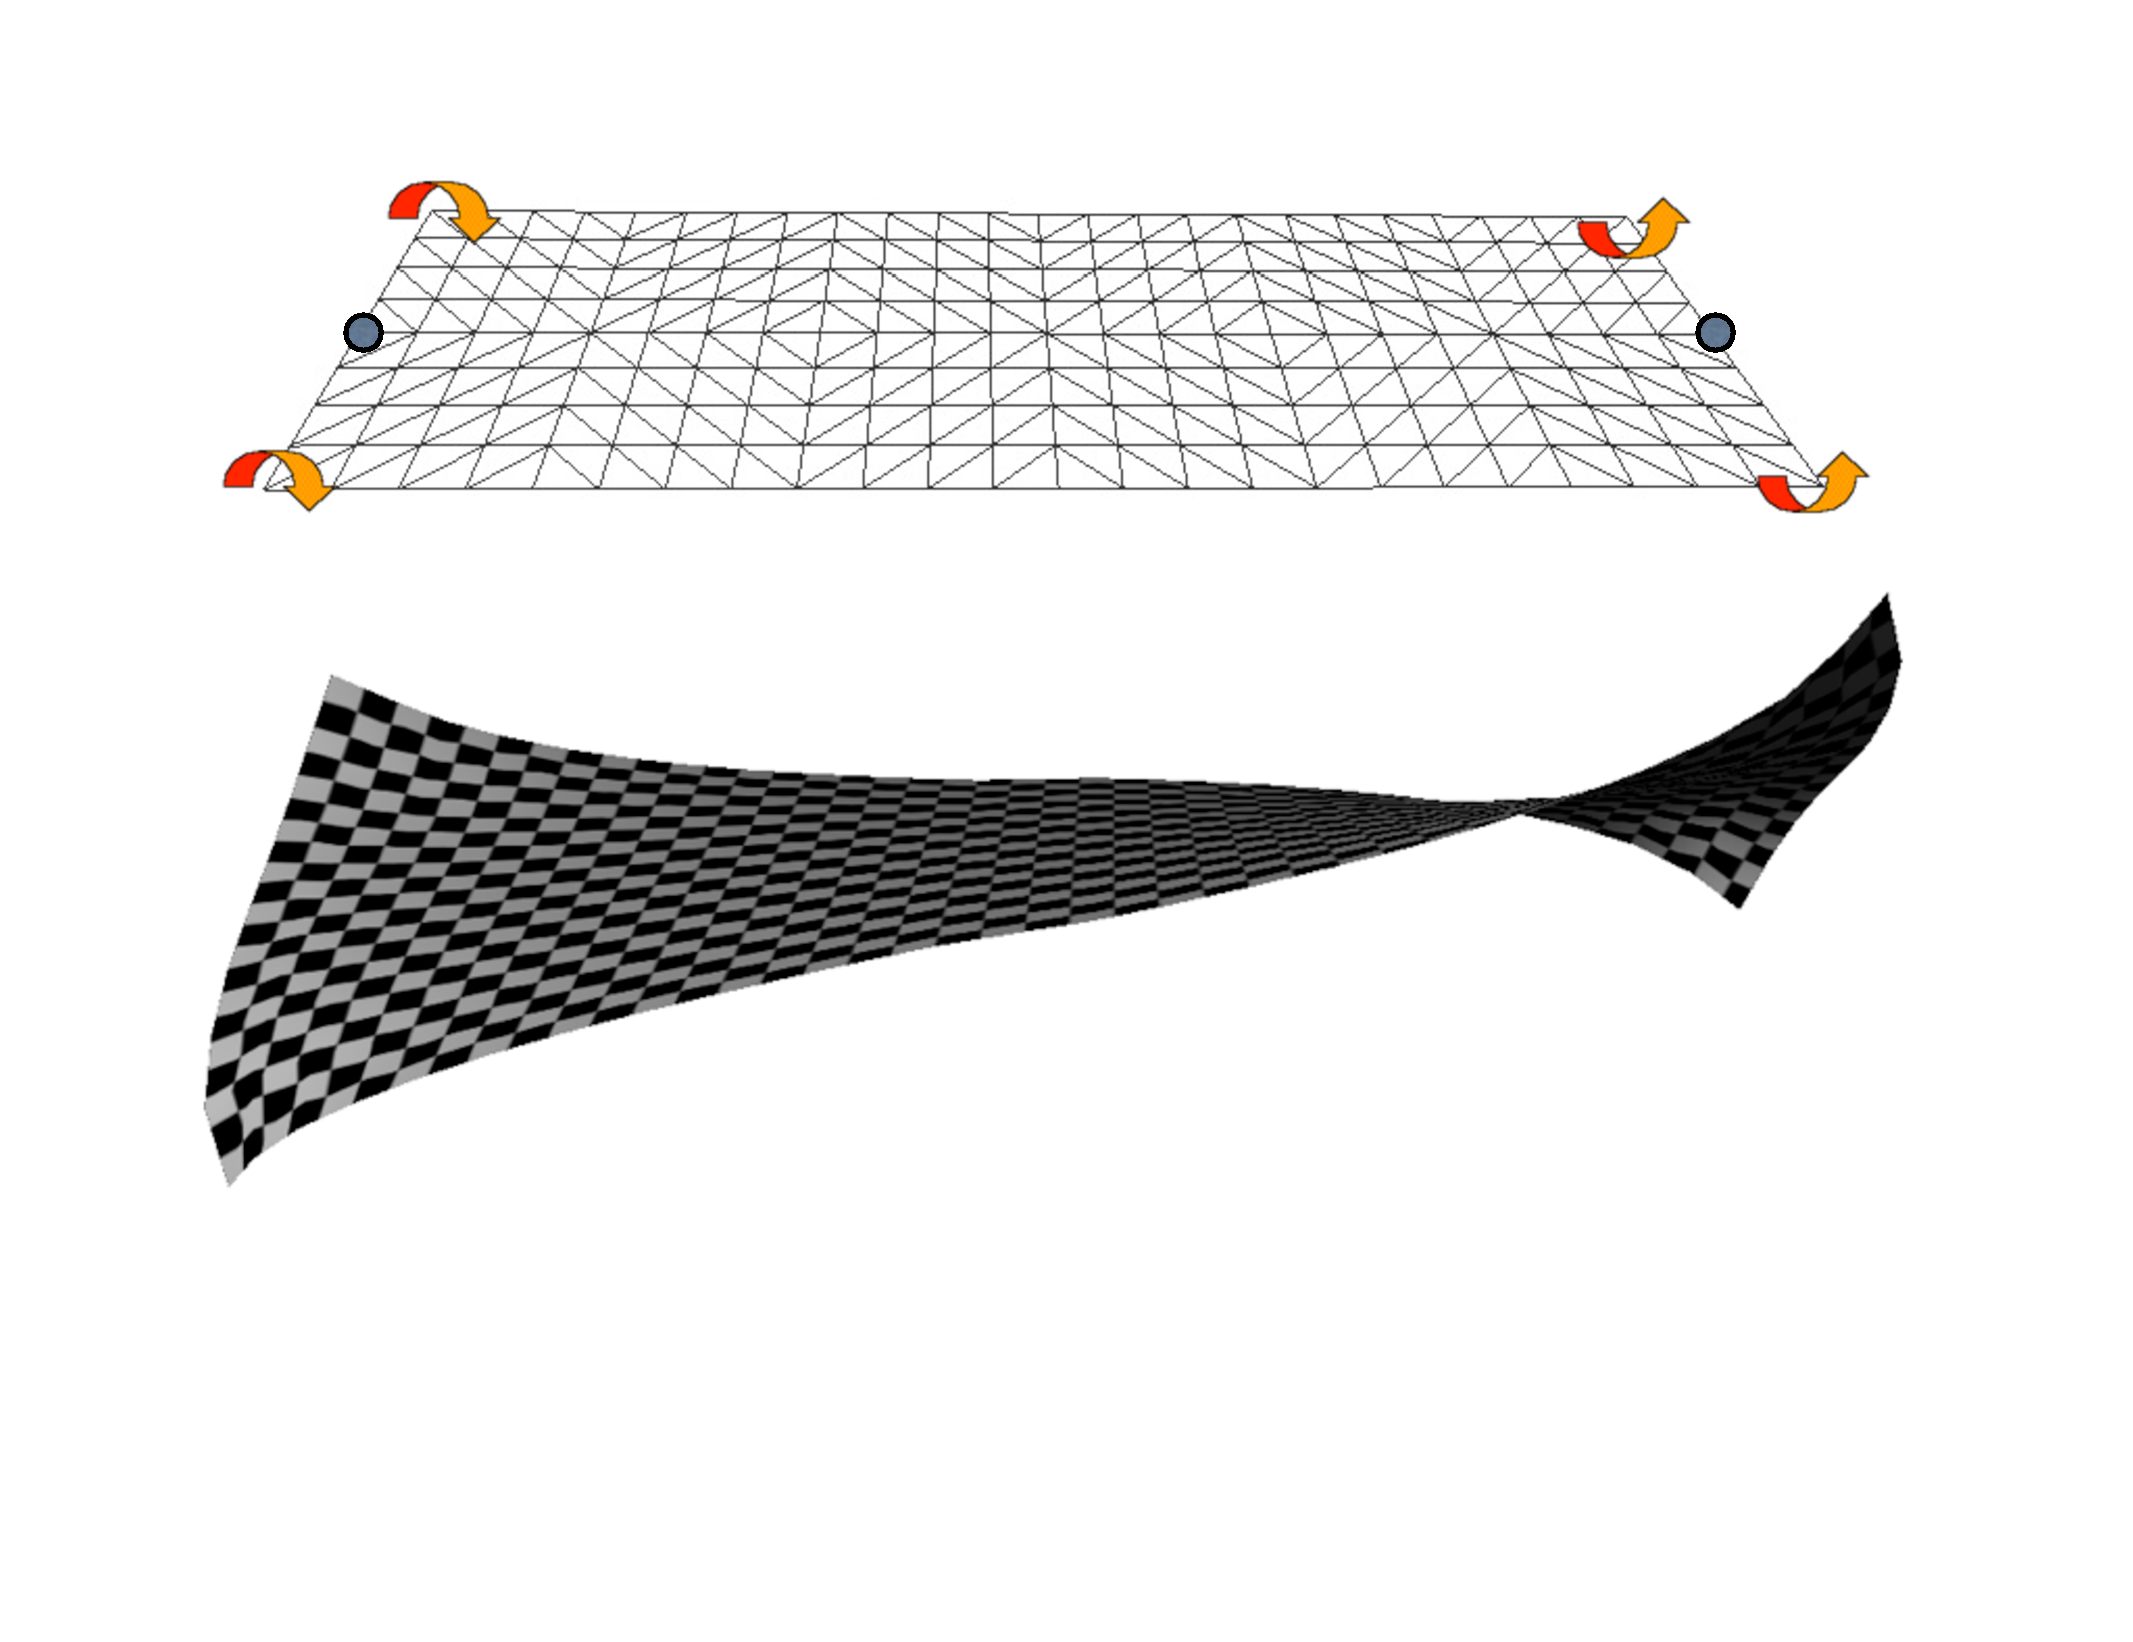
\includegraphics[width=6cm]{images/board_twist}
\caption{Illustration of a key difference between various models of thin objects. While thin plate theory allows to describe bending (left), it cannot represent more complex deformations such as twist (right) which is captured by shell theory.}
\label{fig-boards}
\end{center}
\end{figure}

Development of a satisfactory physical model that runs in real-time but produces visually convincing animation of thin objects has been a challenge in Computer Graphics, particularly in the area of cloth modelling. Rather than resorting to shell theory which involves the most complex formulations in continuum mechanics, previous works have often relied on discrete formulations. Early approaches to cloth modelling only considered in-plane deformation, and often relied on mass-spring models (see \cite{Provot95}, \cite{Hammer08} or \cite{Yu08} for instance). 
More recent works have considered adding bending through angular springs. For instance Taskiran \emph{et al.} \cite{Taskiran05} have chosen to use a linear representation of angular springs to supply bending and torsion effects in hair modelling, which allowed them to simulate curly hair with good realism. Wang \emph{et al.} \cite{Wang07} successfully used a network of linear and angular springs to describe bending and twisting of catheters and guidewires in an interventional radiology simulator. 
Yet, such models are limited in their ability to describe certain behaviour, as they do not rely on continuum mechanics. Another limitation of such models is the difficulty to derive spring stiffness (in particular for angular springs) from elastic properties (Young's modulus and Poisson's ratio). For these reasons, other approaches have been proposed. Among the different models introduced recently we can mention the work of Choi \emph{et al.} \cite{Choi07} and Bridson \emph{et al} \cite{Bridson03}. Choi \emph{et al.} proposed a real-time simulation technique for thin shells undergoing large deformations. The authors adopt the energy functions from the discrete shells proposed by \cite{Grinspun03}. For real-time integration of the governing equation, they adapted a modal analysis technique, called modal warping. The resulting simulations run in real-time even for large meshes, and the model can handle large bending and/or twisting deformations with acceptable realism. Bridson \emph{et al.} followed the same energy approach to derive their bending model but improved the resolution of the equations by suggesting a novel mixed implicit/explicit integration scheme. They also presented a post-processing method for treating cloth-character collisions that preserves folds and wrinkles. Pabst \emph{et al.} improved the bending modelling used by Bridson \emph{et al.} to allow the integration of measured material data. A method to use thin shell dynamics with point sampled surfaces for efficient animation was recently proposed by Wicke \emph{et al.} \cite{Wicke05} where the curvature of the shell is measured through the use of fibers.

In this paper we consider the problem of lens implant folding, unfolding and deployment within a very constrained space. An important difference with previous works is that the ratio stiffness / mass of artificial lenses is very high compared to many material (such as fabric), resulting in added difficulties to obtain a numerically stable simulation. Indeed, if the mass density of cotton and acrylic is about the same, the stiffness of intra-ocular implants is three orders of magnitude higher. The closest work to what we propose is the one of Thomaszewski \emph{et al.} \cite{Thomaszewski06} who derive their formulation from thin shell analysis in a co-rotational framework. However, the authors use very soft and deformable material (Young's modulus $E = 5000\,Pa$ and Poisson's ratio $\nu = 0.25$).

\section{Co-rotational triangular shell model}

We propose to define a triangular shell element by combining a two-dimensional in-plane membrane energy, with an off-plane energy for describing bending and twist (see figure \ref{fig-triangle}). To allow for real-time simulation, a computationally efficient formulation is needed. We therefore propose to extend the co-rotational idea introduced by Fellippa in \cite{Felippa00}. Indeed co-rotational approaches have been successfully applied to real-time simulation of volumetric objects over the last few years \cite{Muller04}. They offer a good trade-off between computational efficiency and accuracy by allowing small deformations but large displacements. We propose to improve and extend a plate model first introduced by Przemieniecki \cite{Przemieniecki68} to a co-rotational formulation. Once combined with an in-plane membrane formulation we obtain an accurate, yet computationally efficient, shell finite element method featuring both membrane and bending energies. 

\begin{figure}
\centering
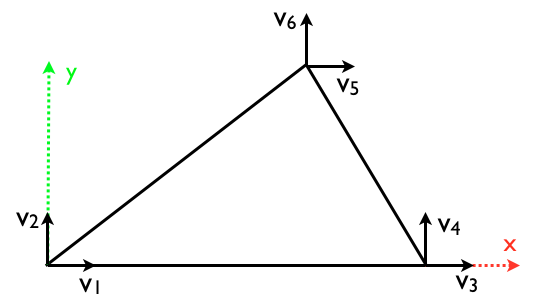
\includegraphics[height=3cm]{images/triangle_membrane}
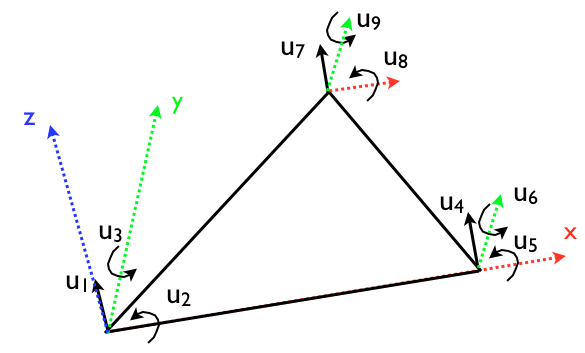
\includegraphics[height=3.5cm]{images/triangle_bending}
\caption {A triangular shell element can be defined as a combination of a triangular in-plane membrane element (left) and a triangular thin plate in bending (right). The different degrees of freedom $v$ and $u$ of both models are illustrated above.}
\label{fig-triangle}
\end{figure}

\subsection{Triangular elastic membrane}

The computation of the triangular elastic membrane stiffness matrix can be derived from previous works dealing with tetrahedral co-rotational elements (see Muller \emph{et al.} \cite{Muller04} for instance). The element stiffness matrix $\textbf{K}_e$ can be computed as follows:

\begin{equation}
\textbf{K}_e = \int_v \textbf{J} \boldsymbol\chi \textbf{J}^{T} dV
\end{equation}

where $\textbf{J}$ is the strain-displacement matrix and $\boldsymbol\chi$ embodies the material's behaviour. The implant is very stiff and we therefore assume that the local deformations remain limited during the deployment and a linear constitutive law is sufficient. Thus in the simple case of Hooke's law we have:

\begin{equation}
\boldsymbol\chi = \frac{E}{12(1-\nu^2)}
\begin{bmatrix}
1 & \nu & 0 \\
\nu & 1 & 0 \\
0 & 0 & \frac{1}{2} (1-\nu)
\end{bmatrix}
\end{equation}

The stiffness matrix in the global frame is eventually obtained using the rotation matrix of the element: $\textbf{K} = \textbf{R} \textbf{K}_e \textbf{R}^{T}$ where $\textbf{R}$ describes the rotation of the (triangular) element with respect to its initial configuration.

\subsection{Triangular plate bending}

To calculate the stiffness matrix for the transverse deflections and rotations shown on figure \ref{fig-triangle}, we start with the assumed deflection $u_z$ of the form
\begin{equation}
 u_z = c_1 + c_2x + c_3y + c_4x^2 + c_5xy + c_6y^2 + c_7x^3 + c_8xy^2 + c_9y^3
\label{eq-deflection}
\end{equation} 

where $c_1$, \ldots , $c_9$ are constants. Equation~\ref{eq-deflection} solves an issue of symmetry which was observed with the deflection function proposed by Przemieniecki in \cite{Przemieniecki68}. These constants can be evaluated in terms of the displacements and slopes at the three corners of the triangular plate using 
\begin{equation}
\textbf{u} = \textbf{Cc}
\label{eq-U}
\end{equation} 
where $\textbf{u} = \left\{u_1 u_2 \ldots u_9 \right\} $ and $\textbf{c} = \left\{c_1 c_2 \ldots c_9 \right\} $. Matrix $\textbf{C}$ derives from equation~\ref{eq-U}:
\begin{equation}
C = 
	\begin{bmatrix}
	1 & 0 & 0 & 0 & 0 & 0 & 0 & 0 & 0 \\
 	0 & 0 & 1 & 0 & 0 & 0 & 0 & 0 & 0 \\
	0 & -1 & 0 & 0 & 0 & 0 & 0 & 0 & 0 \\
	1 & x_2 & 0 & x_2^2 & 0 & 0 & x_2^3 & 0 & 0 \\
	0 & 0 & 1 & 0 & x_2 & 0 & 0 & 0 & 0 \\
	0 & -1 & 0 & -2x_2 & 0 & 0 & -3x_2 & 0 & 0 \\
	1 & x_3 & y_3 & x_3^2 & x_3y_3 & y_3^2 & x_3^2 & x_3y_3^2& y_3^3 \\
	0 & 0 & 1 & 0 & x_3 & 2y_3 & 0 & 2x_3y_3 & 3y_3^2 \\
	0 & -1 & 0 & -2x_3 & -y_3 & 0 & -3x_3^2 & -y_3^2 & 0
	\end{bmatrix}
\end{equation} 
The notations 
\begin{equation}
u_1 = (u_z)_{x_1,y_1} \hspace{1cm} u_2 = \left(\frac{\partial u_z}{\partial y}\right)_{x_1,y_1} \hspace{1cm} u_3 = - \left(\frac{\partial u_z}{\partial x}\right)_{x_1,y_1}
\end{equation} 
and so on for the two other vertices, were used.

We can calculate the strains from the flat-plate theory using:
\begin{equation}
e_{xx} = -z \frac{\partial^2u_z}{\partial x^2}
\end{equation} 
\begin{equation}
e_{yy} = -z \frac{\partial^2u_z}{\partial y^2}
\end{equation} 
\begin{equation}
e_{xy} = -2z \frac{\partial^2u_z}{\partial x \partial y}
\end{equation} 

Hence, using the above equations and equation (\ref{eq-deflection}), we have
\begin{equation}
\begin{bmatrix}
e_{xx} \\
e_{yy} \\
e_{xy}
\end{bmatrix}
= 
-z
\begin{bmatrix}
0 & 0 & 0 & 2 & 0 & 0 & 6x & 0 & 0 \\
0 & 0 & 0 & 0 & 0 & 2 & 0 & 2x & 6y \\
0 & 0 & 0 & 0 & 2 & 0 & 0 & 4y & 0 \\
\end{bmatrix}
\textbf{c}
\label{eq-strains}
\end{equation} 
or symbolically $\textbf{e} = \textbf{Dc}$ where $\textbf{D}$ stands for the $3\times 9$ matrix in equation \ref{eq-strains}, including the pre-multiplying constant $-z$. Noting from equation (\ref{eq-U}) that $\textbf{c} = \textbf{C}^{-1}\textbf{u}$, we have:
\begin{equation}
\textbf{e} = \textbf{DC}^{-1}\textbf{u} = \textbf{bu}
\end{equation} 
where $\textbf{b} = \textbf{DC}^{-1}$. 
Knowing that the stiffness matrix $\textbf{K}_e$ for an element is obtained from
\begin{equation}
\textbf{K}_e = \int_v \textbf{b}^{T} \boldsymbol\chi \textbf{b} dV
\end{equation} 
where $\boldsymbol\chi$ is the material matrix, the substitution of $\textbf{b}$ into this expression yields
\begin{equation}
\textbf{K}_e = (\textbf{C}^{-1})^T \int_v \textbf{D}^{T} \boldsymbol\chi \textbf{D} dV \textbf{C}^{-1}
\end{equation} 
The integration is carried out numerically using Gauss points located at the middle of each edge of the triangle. 

\subsection{Implementation}

In practical terms, the different computations associated with each triangular shell element can be described as follows:
%
\begin{enumerate}
\item Compute the rotation matrix $\textbf{R}$ from global to triangle (local) frame
\item Compute the local displacement vector $\textbf{u} = \{v_1, v_2, 0, u_2, u_3, v_3, v_4, 0, u_5, u_6,$ $v_5, v_6, 0, u_8, u_9 \} $ for each of the 3 nodes of the triangle (the nodes have 6 degrees-of-freedom). As we are in a co-rotational framework the normal displacements $u_1, u_4, u_7$ of all 3 nodes are null in the local frame of the triangle. 
\item Compute matrix $\textbf{D}_i$  at each Gauss point $i$
\item The strain-displacement matrix at each Gauss point $i$ is computed with $\textbf{J}_i = \textbf{D}_i \textbf{C}^{-1}$
\item Compute the local stiffness matrix $\textbf{K}_e$ of the element as $\textbf{K}_e = \displaystyle{\sum^3_{i=1}} \textbf{J}_i \boldsymbol\chi \textbf{J}_i^T$
\item Transform the local element stiffness matrix into the global frame and add it to a global stiffness matrix
\end{enumerate}

The co-rotational shell formulation has been successfully implemented into the open-source framework SOFA \cite{SOFA}. 

\subsection{Validation}

We compared our model with some theoretical results reported by Zhongnian \cite{Zhongnian86} to assess its quality in modelling bending. The test that we carried out uses a square shape mesh clamped on all four edges. A uniform load is then applied on the square and the maximum deflection $z_{max}$ at the centre can be calculated. Several simulations are performed with increasing load values $q$ (ranging from $1$ to $5 N/m^2$) and the following parameters were used: Young's Modulus $E = 1.092 \times 10^6 \,Pa$, Poisson's ratio $\nu = 0.3$, square edge length $L = 10\,m$, thickness $h = 0.1\,m$. Using these particular values it can be shown that $z_{max} = 0.126\,q$. The maximum deflection obtained in our simulations are reported in table \ref{tab-results}. In average we found $z_{max} = 0.1248\,q $, resulting in a $0.93\,\%$ error between our model and theoretical results on that test. 

\begin{table}[ht]
	\centering
	\begin{tabular}{p{9cm}|c|c|}
	\cline{2-3}
	\multirow{5}{*}{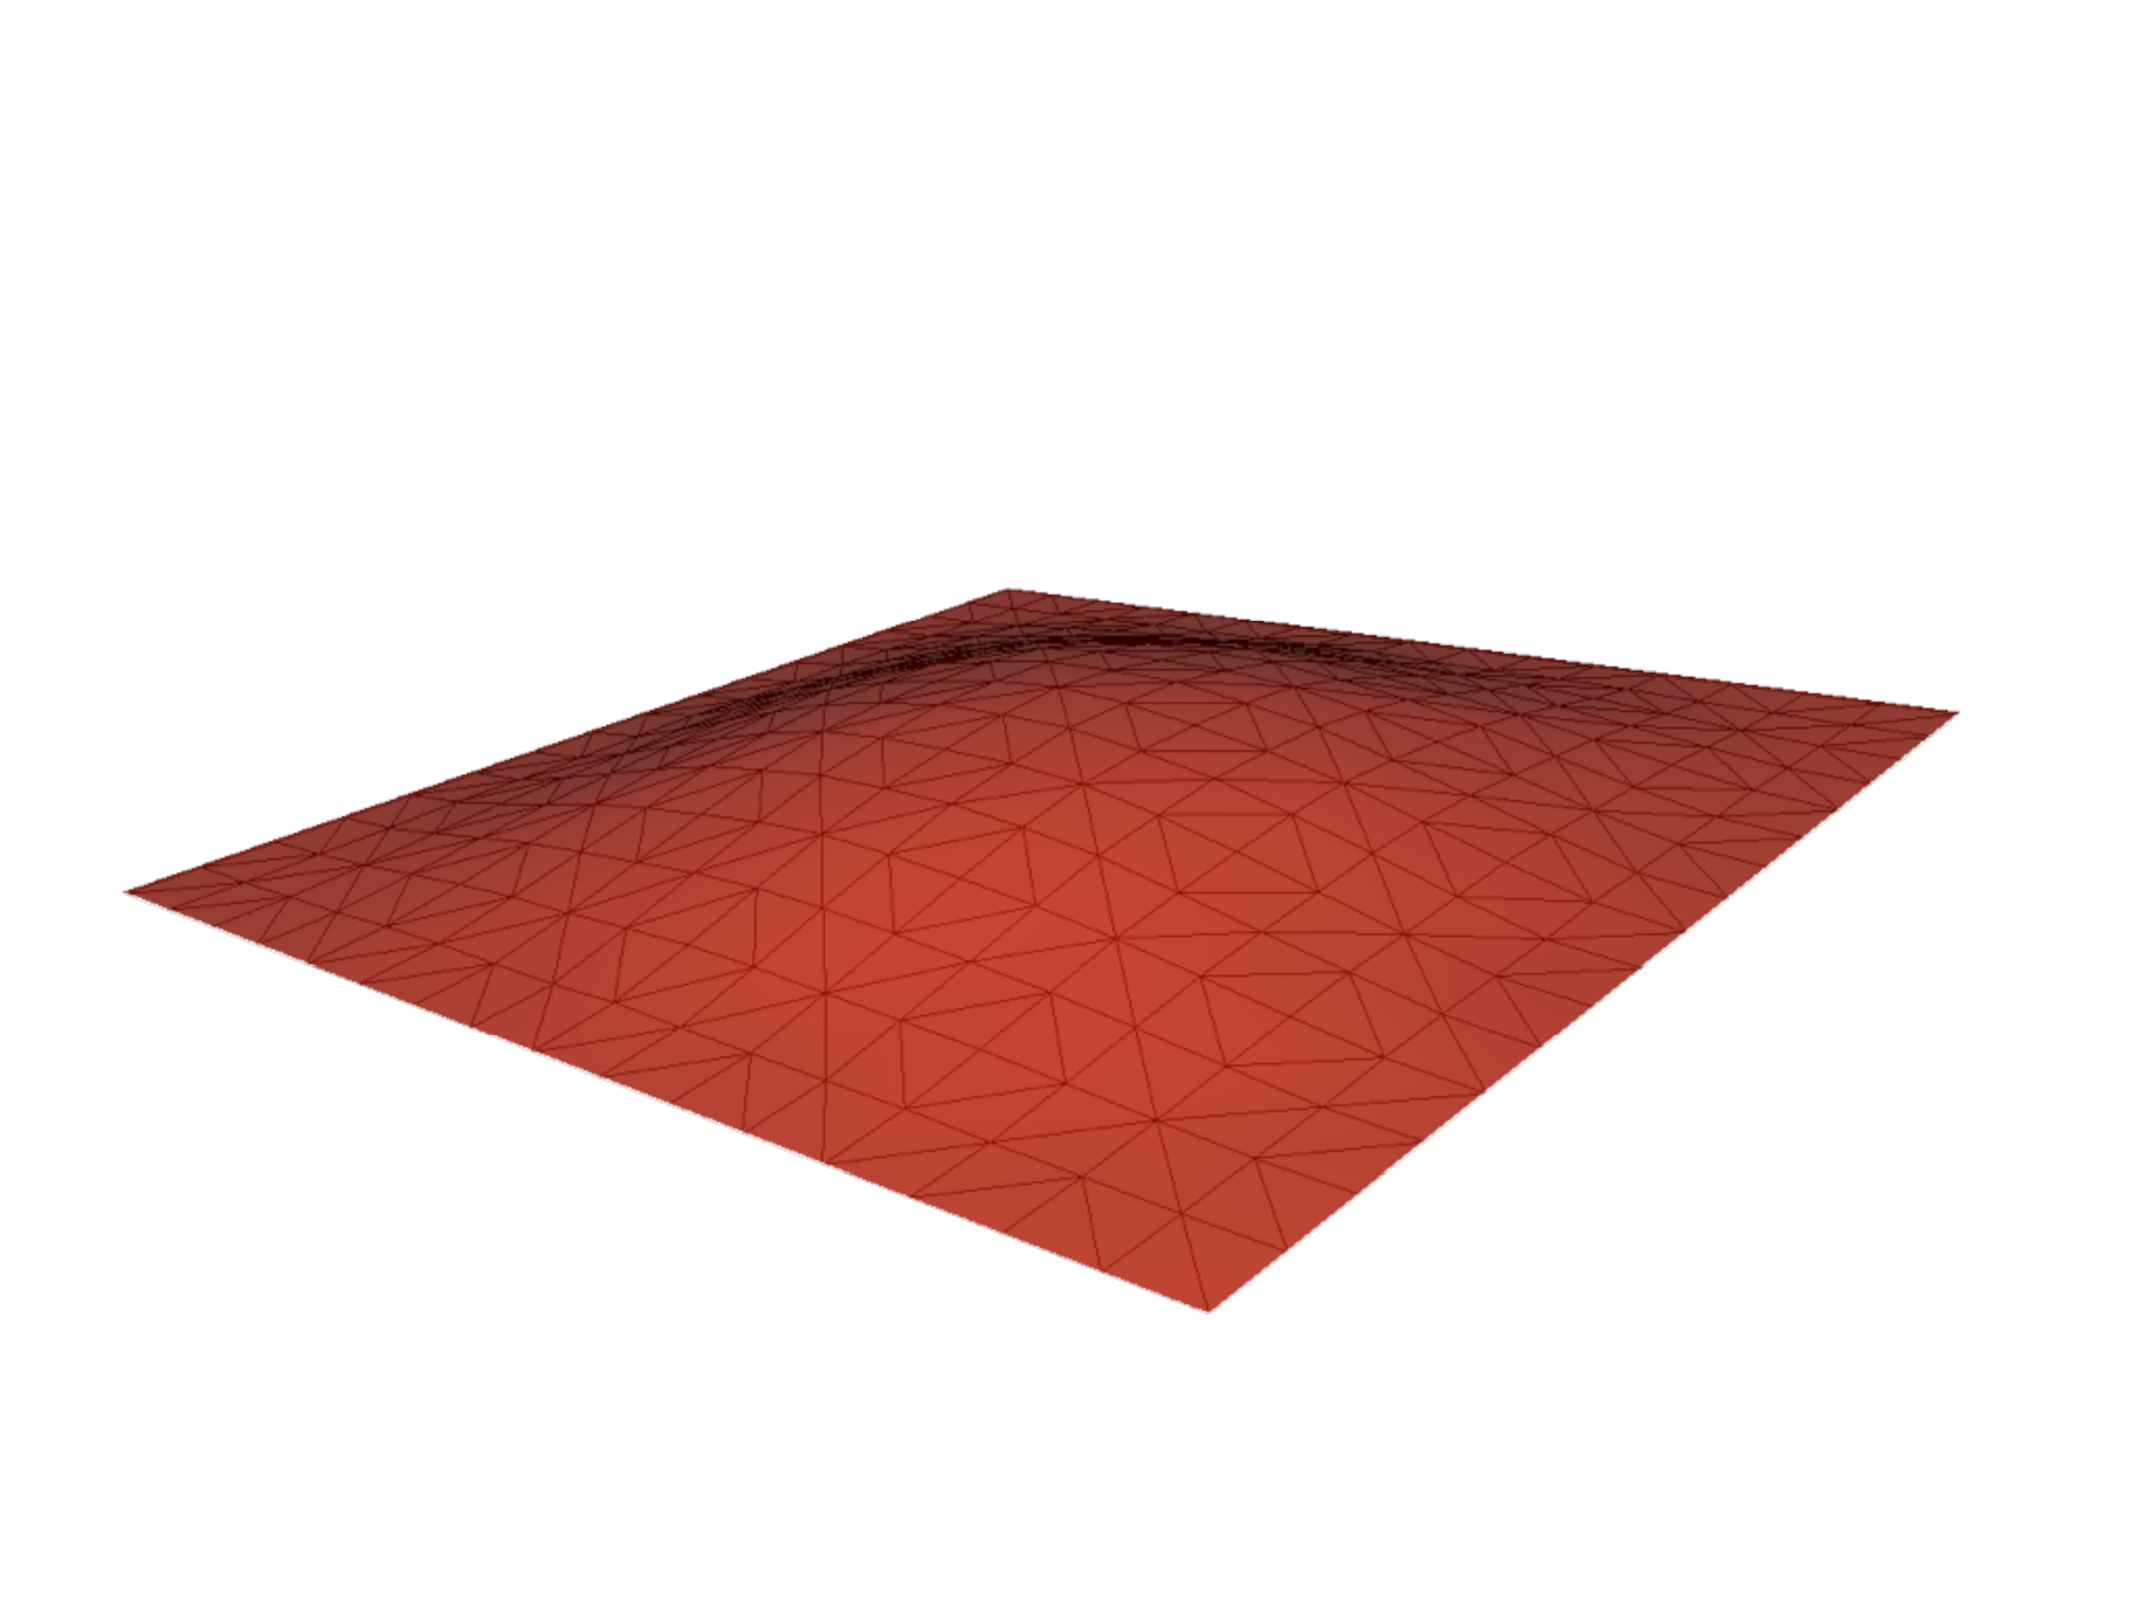
\includegraphics[height=3.5cm]{images/clamped_square}} & $q$ & $z_{max}$ \tabularnewline
	\cline{2-3}
	& $\,1\,$ & $\, 0.1218 \,$ \tabularnewline
	& $\,2\,$ & $\, 0.2475 \,$ \tabularnewline		
	& $\,3\,$ & $\, 0.3747 \,$ \tabularnewline	
	& $\,4\,$ & $\, 0.5050 \,$ \tabularnewline		
	& $\,5\,$ & $\, 0.6374 \,$ \tabularnewline
	\cline{2-3}
	\end{tabular}
	\vspace{1cm}
	\caption{Comparison of our shell model with theoretical results on the bending of a square plate. An error of less than $1\,\%$ was found between our simulation and theoretical results.}
	\label{tab-results}
\end{table}

\section{Simulation of the intra-ocular lens injection}

%Cataract surgery is the removal of the natural lens of the eye (also called \emph{crystalline lens}) that has developed an opacification, which is referred to as a cataract. Metabolic changes of the crystalline lens fibers over the time lead to the development of the cataract and loss of transparency, causing impairment or loss of vision. During cataract surgery, a patient's cloudy natural lens is removed and replaced with a synthetic lens to restore the lens' transparency (figure \ref{fig-surgery}). The last step in the simulation of this surgery is the injection of the implant and its deployment within the lens capsule.

Cataract surgery consists in three main steps: capsulorhexis, phacoemulsification, and implantation of an intra-ocular lens. Prior to starting the surgery, a viscoelastic fluid is introduced into the capsule to facilitate capsulorhexis creation and provide protection during phacoemulsification. This fluid remains in the capsule for the duration of the surgery, including the injection of the implant. Capsulorhexis is the technique used to remove a part of the anterior lens capsule. Phacoemulsification consists in using a surgical device which tip vibrates at an ultrasonic frequency to emulsify the natural lens material and then aspirate the  fragments of the cortical material. After the removal of the diseased lens, an intra-ocular lens is implanted into the eye, through a small incision (about 2 mm) using a foldable intra-ocular lens (see figure \ref{fig-surgery}). The foldable lens, usually made of acrylic material, is then implanted within the lens capsule through the incision used during phacoemulsification. In some cases the implant can be flipped or  the hooks (also called \emph{haptics}) can break. Therefore the simulation of the insertion and deployment of the implant is crucial for achieving a successful surgery.

\begin{figure}[h]
\begin{center}
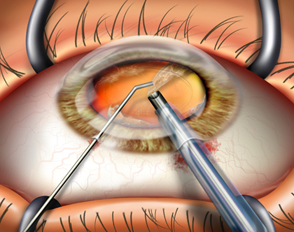
\includegraphics[height=3.2cm]{images/suction}
\hfill
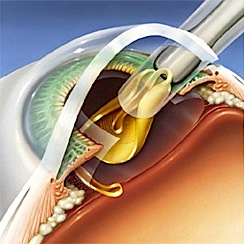
\includegraphics[height=3.2cm]{images/implant_injection_step_1}
\hfill
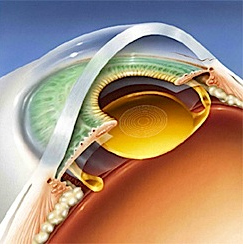
\includegraphics[height=3.2cm]{images/implant_injection_step_2}
\caption [Cataract surgery] {Left: removal of the opacified lens by phacoemulsification. Center: insertion of the lens implant which is folded inside the injection device and then deploys within the lens capsule. Right: the lens in place in the capsule.}
\label{fig-surgery}
\end{center}
\end{figure}

To simulate the insertion and deployment of an intra-ocular lens, we first created a triangulation of the lens surface. Particular care was given to the mesh, to ensure that areas where large stresses occur contain a higher density of elements (figure \ref{fig-mesh}). This was done by noting the constraints applied by the surgeon to the haptics while inserting the implant within the injection device. During this stage, the haptics are folded onto the implant body, leading to high stresses at the junctions. The lens mesh contains $743$ triangles and $473$ nodes. Models of the injection device and the entire eye anatomy were also created. Physical parameters of the lens implant have been provided by the manufacturer Alcon and they are presented in table \ref{tab-parameters}.

\begin{table}[h!]
	\begin{center}
		\begin{tabular}{|p{3cm}|p{3cm}|p{3cm}|}
		\hline
		 \centering Young's modulus & \centering Poisson's ratio & \centering Mass density \tabularnewline
		\hline
		\centering $1 MPa$ & \centering $0.42$ & \centering $1.2 g/cm^3$ \tabularnewline
		\hline
		\end{tabular}
	\vspace{0.3cm}
	\caption{Physical parameters of the intra-ocular implant (source: Alcon)}
	\label{tab-parameters}
	\end{center}
\end{table}

The first difficulty is to obtain the folded geometry of the lens within the injection device. This step is not important for the training process and does not need to be interactive. Indeed the surgeon does not always have to prepare the implant as some injection devices are readily available with a folded implant already in place. We simulate the folding process by first folding the haptics onto the implant body. The body was then bent while keeping the haptics inside to obtain the shape described in figure \ref{fig-implantFolding}. The whole process was carried out by applying the necessary forces and boundary conditions on the body and haptics of the implant. The folded implant was then placed into the injection device. The simulation of the injection consists in pushing the intra-ocular implant within the injection device into the lens capsule. During these stages of the simulation, complex contacts occur and consist of self collisions of the lens as well as collisions between the lens and the injector and later with the capsule. To solve the contacts we use the contact warping method proposed Saupin \emph{et al.} \cite{Saupin08} as it offers an efficient way to compute physically correct contact responses in the case of co-rotational models. As adhesions between the haptics and the body is often observed in surgery, friction is also taken into account in the contact response process.

\begin{figure}[!h]
\centering
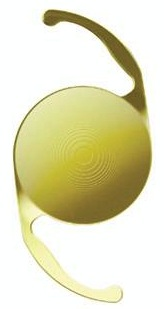
\includegraphics[height=5cm]{images/IOL}
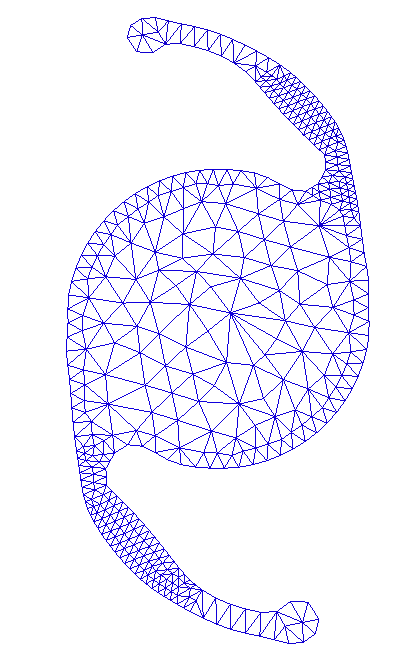
\includegraphics[height=5cm]{images/mesh_implant}
\caption [Lens implant and its mesh] {An actual intra-ocular implant and the triangular mesh used in our simulations. Notice the higher density of elements in areas where large deformations will take place.}
\label{fig-mesh}
\end{figure}

\begin{figure}[!h]
\centering
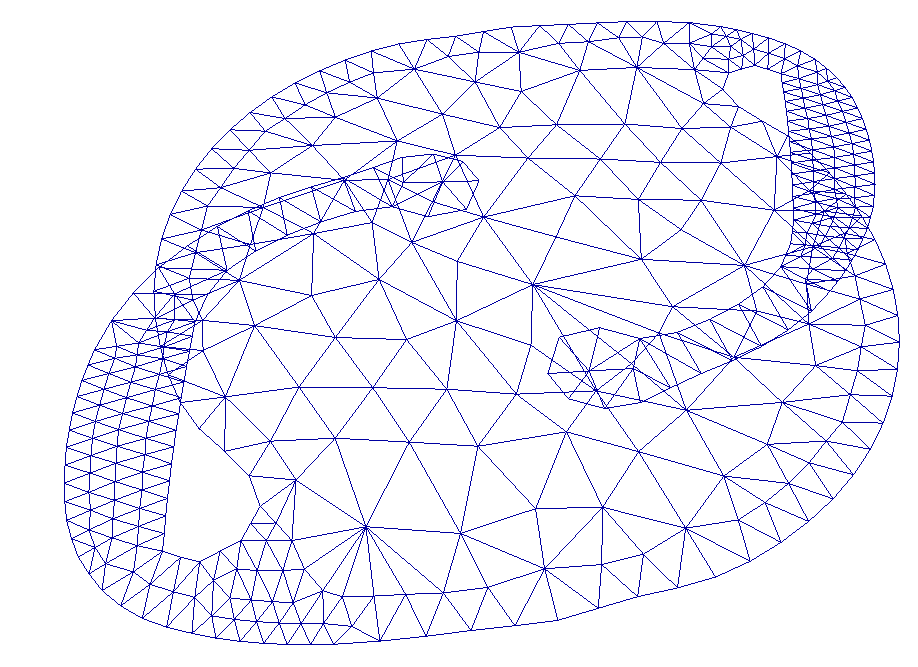
\includegraphics[width=4cm]{images/implant_folding1}
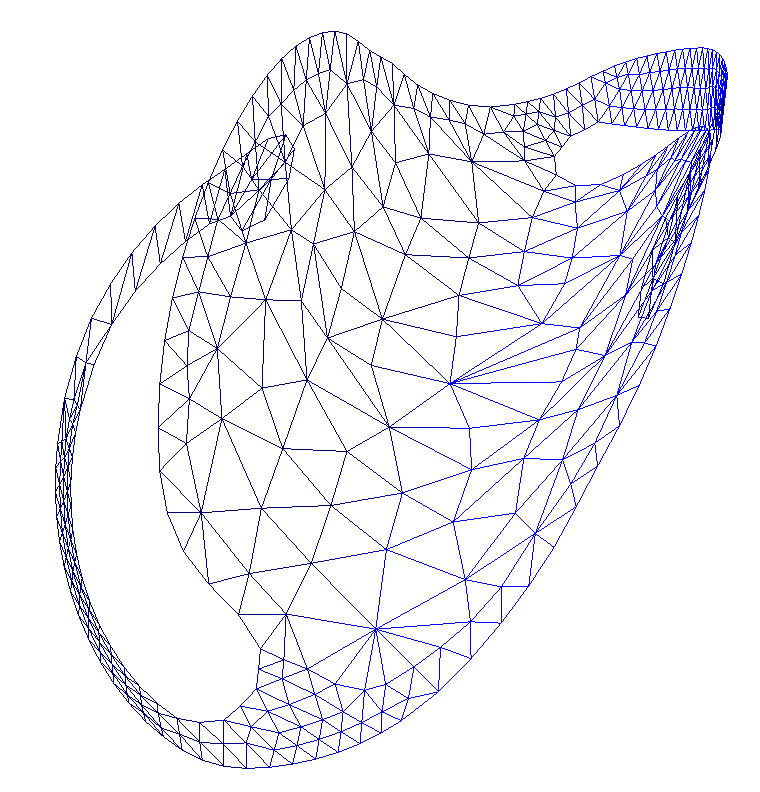
\includegraphics[width=3.5cm]{images/implant_folding2} \\
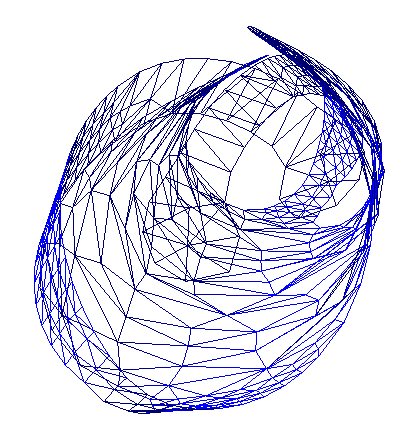
\includegraphics[width=3cm]{images/implant_folding3}
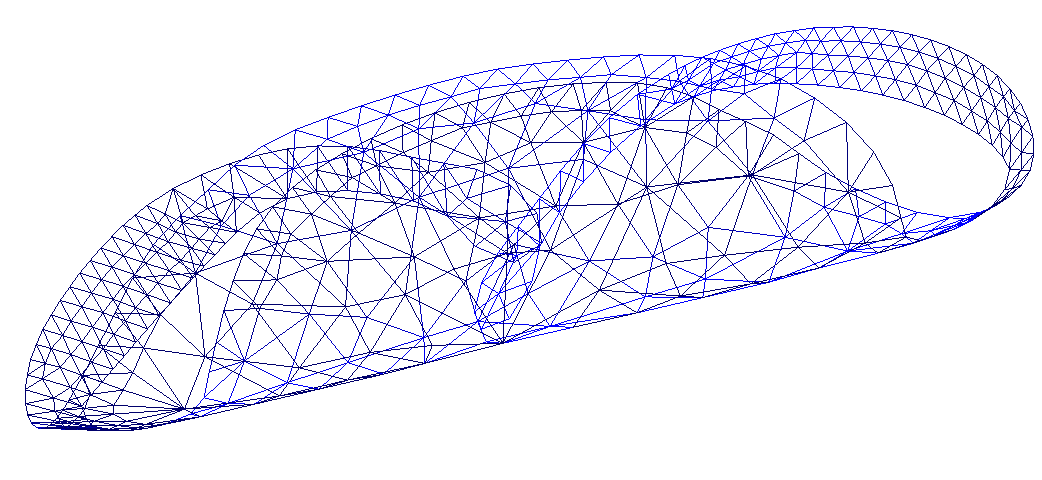
\includegraphics[width=5.5cm]{images/implant_folding4}
\caption [Folding of intra-ocular implant] {Top: intermediary steps of the intra-ocular implant folding. Bottom: fully folded implant ready to be placed into the injection device.}
\label{fig-implantFolding}
\end{figure}

Results of our simulation are illustrated in figure \ref{fig-simu-results}. We can notice the progressive deployment of the implant when it exits the injector.  The shape of the intra-ocular lens remains very close to that of a real one during all stages of the simulation: within the injector, during the ejection phase, and when in place within the capsule. Due to the high stiffness and low mass of the lens, a direct sparse solver was used at each time step (dt $= 0.01$\,s) rather than an iterative solver, resulting in a more accurate and more stable simulation, to the detriment of computation times (about 5 FPS for the complete simulation, and about 10 FPS for the deformation only, on a 2.4 GHz processor).

\begin{figure}[!h]
\centering
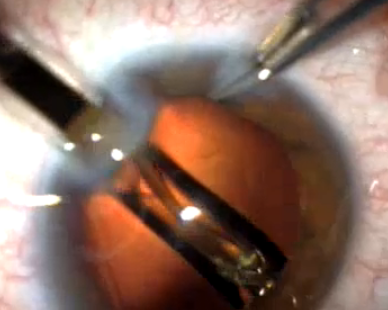
\includegraphics[width=4cm]{images/surgery1}
\hfill
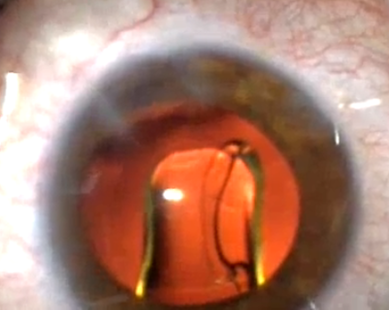
\includegraphics[width=4cm]{images/surgery2}
\hfill
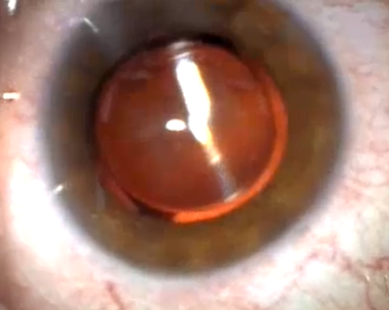
\includegraphics[width=4cm]{images/surgery3} \\
\vspace{0.1cm}
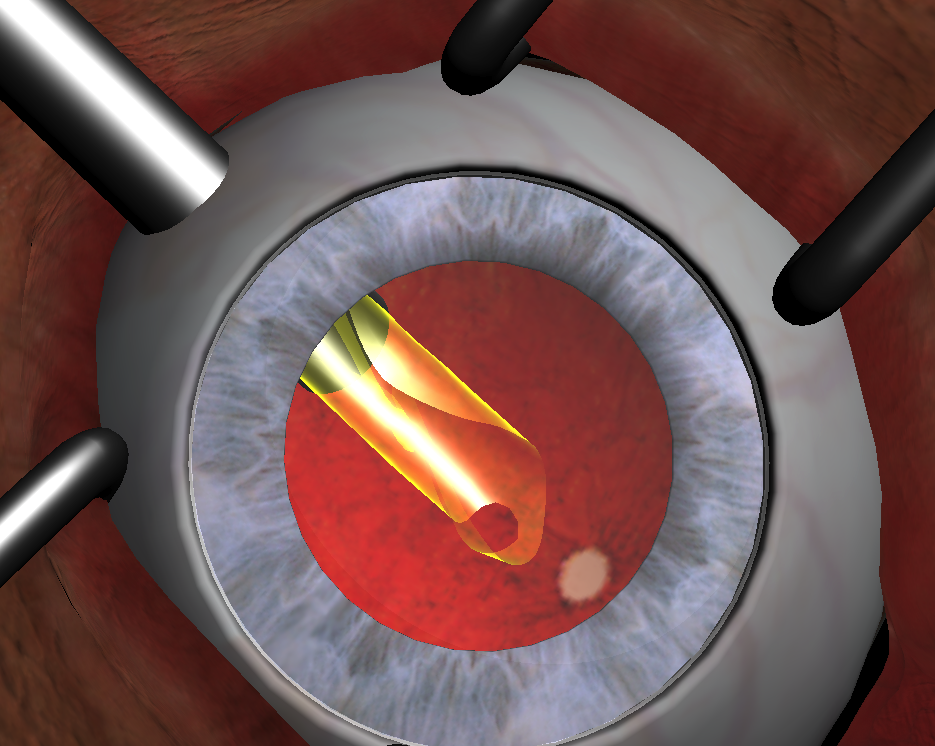
\includegraphics[width=4cm]{images/simu1}
\hfill
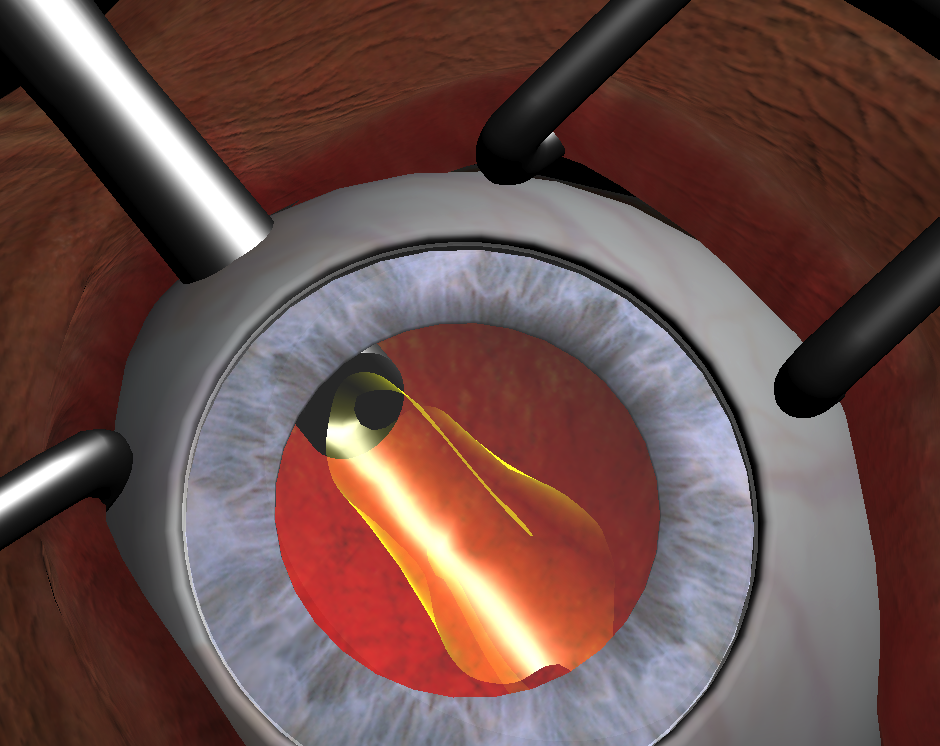
\includegraphics[width=4cm]{images/simu2}
\hfill
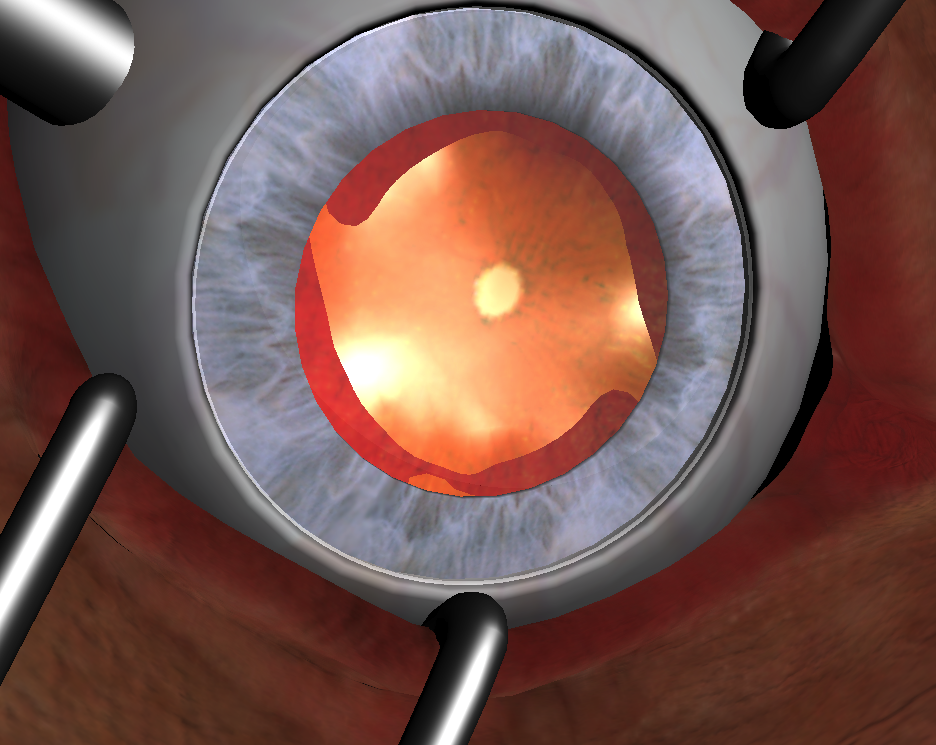
\includegraphics[width=4cm]{images/simu3}
\caption [Lens imlant] {Three steps of the simulation of the intra-ocular lens implant injection and its deployment within the lens capsule. Top: images from a real cataract surgery, courtesy of Dr. Tarek Youssef, ophtalmologist in Canada. Below: our simulation of the implant's deployment.}
\label{fig-simu-results}
\end{figure}

\section{Conclusion}

We proposed a co-rotational formulation for shell elements by extending a classical in-plane triangular finite element approach. This simple shell element can efficiently handle both membrane, bending and twist forces. The validity of our approach has been demonstrated though comparison with theoretical results. It was then applied it to a rather complex application: the simulation of intra-ocular lens implant deployment in a cataract surgery simulation. These preliminary results are very encouraging and show the potential of such models. Examples include the modelling of hollow anatomical structures (stomach, colon, etc.), the simulation of cardiac valve leaflets, and blood vessels. Regarding improvements of our current model and simulation, we plan to account for the interaction with the viscoelastic fluid (currently approximated by a high damping). Computation times also need to be improved through the use of more optimised meshes and by porting our parallelisable algorithm to Graphics Processing Units. 

\section*{Acknowledgments}
We are very grateful to J\'er\'emy Ringard for his invaluable help in improving the eye anatomical model, to J\'er\'emie Dequidt and Damien Marchal for understanding Blender, to Fr\'ederick Roy for his help with SOFA, and Nadia Boubchir for her persistence in motivating us to obtain these results in time. 

\bigskip

We would also like to thank INRIA and the SOFA project, as well as CSIRO Preventative Health National Research Flagship, ICTC, The Australian e-Health Research Centre for their fundings. 

\bibliographystyle{splncs}
\bibliography{bibliography}

\end{document}